\documentclass{standalone}
\usepackage{pgfplots,xcolor}
\pgfplotsset{compat=1.18}

\begin{document}
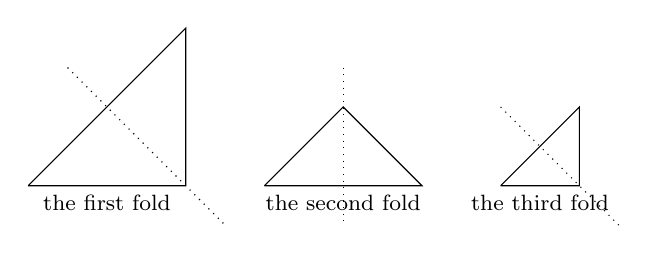
\begin{tikzpicture}
  \begin{scope}[shift={(-1,0)}]
    \draw (0,0) -- (2,0) -- (2,2) -- (0,0);
    \draw[dotted, domain=0.5:2.5] plot ( {\x}, {-\x + 2} );
    \node[below] at (1,0) {\footnotesize the first fold};
  \end{scope}

  \begin{scope}[shift={(2,0)}]
    \draw (0,0) -- (2,0) -- (1,1) -- (0,0);
    \draw[dotted] (1,1.5) -- (1,-0.5);
    \node[below] at (1,0) {\footnotesize the second fold};
  \end{scope}

  \begin{scope}[shift={(5,0)}]
    \draw (0,0) -- (1,0) -- (1,1) -- (0,0);
    \draw[dotted, domain=0:1.5] plot ( {\x}, {-\x + 1} );
    \node[below] at (0.5,0) {\footnotesize the third fold};
  \end{scope}
\end{tikzpicture}
\end{document}
